\documentclass{deimj}
\usepackage[dvipdfmx]{graphicx}
\usepackage[ipaex]{pxchfon}
\usepackage[hyphens]{url}
\usepackage{tabularx}
\usepackage{multirow}

% 印刷位置調整 %
% 必要に応じて値を変更してください.
\hoffset -10mm % <-- 左に 10mm 移動
\voffset -10mm % <-- 上に 10mm 移動

\newcommand{\AmSLaTeX}{%
$\mathcal A$\lower.4ex\hbox{$\!\mathcal M\!$}$\mathcal S$-\LaTeX}
\newcommand{\PS}{{\scshape Post\-Script}}
\def\BibTeX{{\rmfamily B\kern-.05em{\scshape i\kern-.025em b}\kern-.08em
T\kern-.1667em\lower.7ex\hbox{E}\kern-.125em X}}

\papernumber{DEIM Forum 2019 XX-Y}

\jtitle{未訪問エリアの理解支援のための既訪問スポットに基づく類推情報提示手法}
%\jsubtitle{サブタイトル} <- サブタイトルを付けたいときはこの行の先頭の % を取る
\authorlist{%
 \authorentry[em18011@ns.kogakuin.ac.jp]{潘 健太}{KENTA HAN}{UnivN}
 \authorentry[kitayama@cc.kogakuin.ac.jp]{北山 大輔}{DAISUGE KITAYAMA}{UnivN}
 }

\affiliate[UnivN]{工学院大学大学院工学研究科情報学専攻\hskip1zw
  〒163--8677 西新宿1-24-2}
 {School of Engineering,Kogakuin University\\
  1--24--2,Nisisinjyuku,Tokyo,163--8677 Japan}

\begin{document}
\pagestyle{empty}
\begin{jabstract}
近年,観光スポットを決める時にWeb上の観光情報を活用して計画を立てることが多くなっている.しかし,ユーザが多くのエリアから訪問したいエリアを決めた上で,さらに自分のイメージに合う観光スポットを探すのは膨大な時間と労力を必要とする.また,ユーザが未訪問スポットに対して期待と不安を感じる場合がある.
%以前に経験した事柄を,現在直面している事柄あるいは問題にあてはめることを類推と呼ぶ.
本研究では,ユーザの未知なスポットに対する理解を支援するためには,既に訪問したことがある観光スポットの特徴を未訪問スポットにあてはめて理解を支援する類推情報提示を提案する.観光スポット自身の特徴を重視するため,各観光スポットの特徴抽出に,ユーザが入力した観光スポットのすべてのレビュー,対象エリアの観光スポットのすべてのレビューを使用する.また,プロトタイプシステムを構築し,既訪問スポットと未訪問スポットとの類推情報の効果を検証する評価実験を行う.
\end{jabstract}

\begin{jkeyword}
観光スポット,類推,理解支援,レビュー,コサイン類似度,TFIDF,調和平均
\end{jkeyword}
\maketitle


%%%%%%%%%%%%%%%%%%%%%%%%%%%%%%%%%%%%%%%%%%
%%%%%%%%%%%%%%%%%%%%%%%%%%%%%%%%%%%%%%%%%%
\section{はじめに}
\label{sec:Introduction}
%%%%%%%%%%%%%%%%%%%%%%%%%%%%%%%%%%%%%%%%%%
%%%%%%%%%%%%%%%%%%%%%%%%%%%%%%%%%%%%%%%%%%
旅行先を決定する時,旅行者は観光スポット検索サイトや観光情報に関連する書籍を見て観光スポットを選び,旅行計画を立てる.しかし,ユーザにとって訪問したいエリアを決定した後,さらにエリア内に数多く存在する観光スポットから,自身のイメージから外れない観光スポットを見つけることは容易ではない.行きたい観光スポットが決まっていない場合ではランキングやおすすめ情報を見て観光スポットを決めることが多くなると考えられる.この時,ユーザが選択した観光スポットに対するイメージが曖昧になるため不安を感じる場合がある.

近年,観光業とソーシャルネットワーキングサービスの発展スピードが加速しており,体験した観光スポットに対するレビューを観光スポット検索サイトに投稿しているユーザが増加している.さまざまな観光スポットを効果的に理解するためには,既存の情報をもとにして,未知な情報と既知な情報との対応関係を考えることが不可欠となる.この考え方は,以前に経験した事柄(ベースと呼ぶ)を,現在直面している事柄あるいは問題(ターゲットと呼ぶ)にあてはめる類推に相当する.たとえば,金沢の「にし茶屋街」という未知なスポットに対して既訪問の京都の「花見小路」と似ていると説明するとイメージの理解がしやすくすることがある.

本研究では,ユーザの未知なスポットに対する理解を支援するため,既に訪問したことがある観光スポットの特徴を未訪問スポットにあてはめて理解を支援する類推情報提示を提案する.具体的には,ユーザが入力した既訪問スポットと未訪問エリアから,レビュを用いて既訪問スポット内の各スポットの独特な特徴と未訪問エリア内の各スポットの独特な特徴を抽出し,比較を行って類推情報を提示する.このプロトタイプシステムにより,ユーザが未訪問エリアに対する理解の支援を目指す.図\ref{fig:photo_image}は提案手法の概念図である.

本論文の構成は下記のとおりである.2節では関連研究について述べる.3節では提案手法の概要について述べる.4節では構築したプロトタイプシステムの効果を検証する評価実験と考察について述べる.最後に5節では今後のまとめと課題について述べる.

\begin{figure}[t]
  \begin{center}
    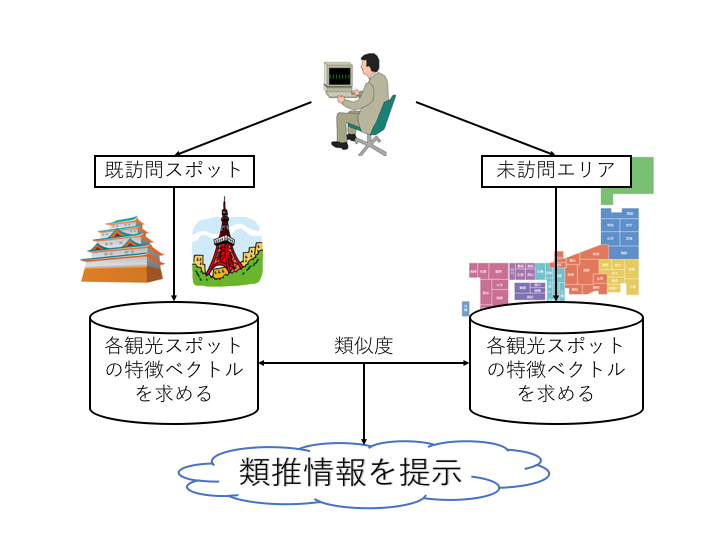
\includegraphics[clip,width=7.0cm]{picture/Photo_Image.png}
    \caption{未訪問エリアの理解支援のための既訪問スポットに基づく類推情報提示手法}
    \label{fig:photo_image}
   \end{center}
\end{figure}


%%%%%%%%%%%%%%%%%%%%%%%%%%%%%%%%%%%%%%%%%%
%%%%%%%%%%%%%%%%%%%%%%%%%%%%%%%%%%%%%%%%%%
\section{関連研究}
\label{sec:Related Research Papers}
%%%%%%%%%%%%%%%%%%%%%%%%%%%%%%%%%%%%%%%%%%
%%%%%%%%%%%%%%%%%%%%%%%%%%%%%%%%%%%%%%%%%%
クチコミを使用した地理情報の検索および推薦に関する研究は数多く行われている.廣嶋ら\cite{Codd01}は,地理情報検索の際のクエリ入力支援として,提示する特徴語の抽出手法について研究を行った.この手法では,各ブログ記事から特徴語候補の抽出および地点の特定を行った.具体的には,特徴語の候補をWikipediaの見出し語に限定し,ポアソン確率を用いて特徴語抽出を行った.

観光地検索するとき,松本ら\cite{Codd02}はクチコミから特徴語を抽出して利用する研究を行なった.抽出対象を任意の名詞として,4種類の手法,TFIDF,ATF(Average Term Frequency),ポアソン確率,エントロピーのうちどの手法が特徴語抽出に適しているのか検討を行なった.また,抽出した特徴語を利用した検索支援システムを試作し,実験を通して特徴語提示の効果を検証した.

上原ら\cite{Codd03}はWebから観光情報を抽出し,複数の特徴ベクトルから観光地間の類似性を評価することで,観光地を推薦するシステムを提案した.観光地の特徴ベクトルは,知恵袋・ブログ上での共起キーワードと時系列分布,知恵袋上でのカテゴリ構造,観光地周辺施設,地図画像から生成した.これらの特徴ベクトルから観光地間の類似度の測定を行い,類似度の高い観光地を推薦した.

野守ら\cite{Codd04}は日本全国の観光地のクチコミデータを用いて,観光客が話題にする観光テーマを確率的に抽出し,そのテーマを軸として各観光地の特徴を定量的に評価した.また,クチコミのテキストデータにテキストマイニングを実行して表現を抽出し,観光地ごとにその表現の出現頻度を集計したクロス集計表にPLSAを実行することで,観光客のクチコミだけに基づいた観光テーマの抽出と観光地の特徴分析を行なった.

類推に関する研究の数多くは,ベースとなる物語とターゲットとなる問題が与えられ,物語の特徴を問題の特徴にマッピングして問題を解決するものである\cite{Codd05}.石田ら\cite{Codd06}は新知識を理解するための類推能力の育成についての研究を行った.具体名詞を明確な事物,抽象名詞を不明確な事物とし,明確な事物をターゲットとして扱う.類推による新知識の理解の枠組みを実装したシステムを利用することで,類推プロセスの理解と繰り返しによる練習を促し,類推能力を育成できるのかについて検証を行った.砂山ら\cite{Codd07}は自身が知っている知識を,その知識を知らない他人に伝える際に,類推を用いて分かりやすく説明するスキルの獲得を支援するシステムを提案した.評価実験により,システムを用いた被験者が,分かりやすい説明を行える能力を身につけられる可能性を確認した.中村ら\cite{Codd08}は新たな概念を創造しようとするとき,本質的な役割を果たす高次認知機能として類推に着目して研究を行った.構造の類似性には3種類あり,特徴の共有数で決まる「対象レベルの類似性」,ベースに存在する関係とターゲットに存在する関係の共有度に基づく「関係レベルの類似性」,および題の解法あるいは目標レベルでの類似性である「プラグマティックな類似性」とがある\cite{Codd09}.

従来のレビューを利用する手法では,クチコミを分析して,対象目標の検索をしやすくための研究が多い.また,類推技術は学習支援でよくて使われている.本研究,提案する未訪問エリアの理解支援のための既訪問スポットに基づく類推情報提示手法は,既訪問スポットと未訪問エリアのレビューを使い,未知ターゲットに対する理解を支援するため,類推の質を明示的扱う.そのため,構造の類似性「関係レベルの類似性」に近いと考えられる.


%%%%%%%%%%%%%%%%%%%%%%%%%%%%%%%%%%%%%%%%%%
%%%%%%%%%%%%%%%%%%%%%%%%%%%%%%%%%%%%%%%%%%
\section{類推情報提示手法}
\label{sec:Analogical Information Presentation Method}
%%%%%%%%%%%%%%%%%%%%%%%%%%%%%%%%%%%%%%%%%%
%%%%%%%%%%%%%%%%%%%%%%%%%%%%%%%%%%%%%%%%%%
我々は,未訪問エリアの理解支援のための既訪問スポットに基づく類推情報提示手法を提案する.具体的にはまず,ユーザが既訪問の複数個の観光スポットと訪問したい観光スポットエリア情報を入力する.既訪問スポットレビューベクトルを使って既訪問スポット毎の特徴ベクトルを求める.未訪問スポットも同様にエリア内の各スポットの特徴ベクトルを求める.次に,既訪問スポットレビューベクトルと未訪問スポットレビューベクトルの差分特徴に類似する特徴を持つ未既訪問観光スポット関連付けを行う.最後に,TFIDFを用いて未訪問エリアの理解支援のための類推情報を定義し,ユーザに提示する.

%%%%%%%%%%%%%%%%%%%%%%%%%%%%%%%%%%%%%%%%%%
\subsection{観光スポットの相対的な特徴}
\label{subsec:Relative features of sightseeing spots}
% 本研究では,観光スポットの特徴を絶対的な特徴と相対的な特徴の2つに分類する.絶対的な特徴とは,観光スポット検索サイトでスポットを検索するためで使う絞り込み情報である.絞り込み情報は例は以下の3つである.
% \begin{itemize}
%  \item カテゴリー:神社・神宮・寺院,観光施設・名所巡り等
%  \item 滞在時間:1時間未満,1\verb|~|2時間等
%  \item 訪問時期:1\verb|~|12月,春,夏,秋等
% \end{itemize}

\begin{figure}[t]
  \begin{center}
    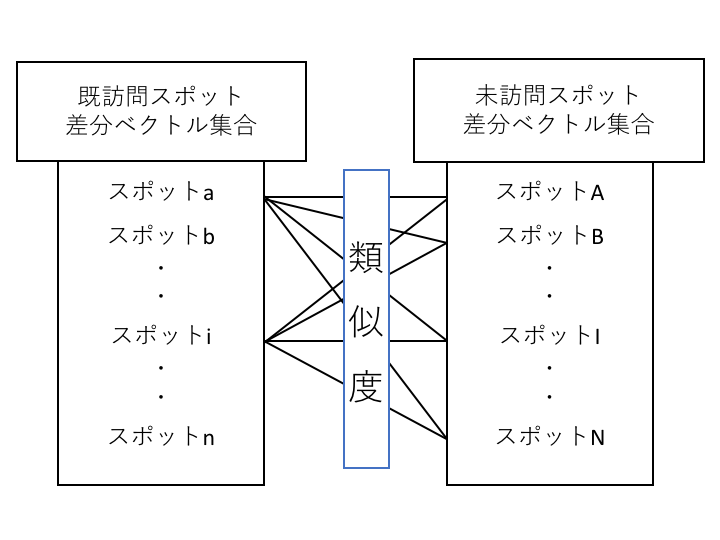
\includegraphics[clip,width=7.0cm]{picture/Photo_CosSim.png}
    \caption{類似度計算概念図}
    \label{fig:photo_exp}
    \end{center}
\end{figure}

本研究では,観光スポットの特徴は相対的な特徴を利用する.相対的な特徴とは,特定の観光スポットが,ある観光スポット集合に含まれた他の観光スポットと比較した場合における独特な特徴である.例として,観光スポット集合内に鹿苑寺と清水寺が存在する場合を考える.このとき鹿苑寺の特徴は,金色,金箔,輝き等となり,清水寺の特徴は,舞台,胎内,一望等となる.どちらも京都に存在する寺院であるため,京都や寺院に関連する特徴は独特な特徴として現れることがない.
次に,観光スポット集合内に東京都庁舎展望台と鹿苑寺が存在する場合を考える.このとき鹿苑寺の特徴は,金閣寺,お寺,金色,京都等となり,東京都庁舎の特徴は,展望,夜景,新宿等となる.観光スポットのカテゴリーが大きく異なる場合であれば,カテゴリーとしての特徴が現れる.また,スポット自身の特徴を表すことができる.本研究では,あるスポットが集合内の他のスポットと比較するとき,より各スポットの特徴を明らかにできる相対的な特徴に着目して研究を行う.

%%%%%%%%%%%%%%%%%%%%%%%%%%%%%%%%%%%%%%%%%%
\subsection{コサイン尺度による類似度計算}
\label{subsec:Calculation of similarity by cosine similarity}
既訪問スポットや未訪問スポットのレビューベクトルは,形態素解析器「mecab-ipadic-NEologd」\footnote{https://github.com/neologd/mecab-ipadic-neologd/}で分かち書き(原型)したレビューを利用して作成する.その後,Doc2Vec\footnote{https://radimrehurek.com/gensim/models/doc2vec.html}のDistributed Bag-of-Wordsを利用して,各スポットの全レビューを使って300次元で作成したベクトルを使う.本稿に置いて,レビューデータは2016年09月末までじゃらん\footnote{https://www.jalan.net/kankou/}から取得したものを用いる.

スポット差分ベクトルは式\ref{math:Vector difference}として定義される.スポット差分ベクトルを求めるスポットを除いたスポット集合の各スポットのスポットベクトルの平均値を引いた値となる.$spot_{set} =\{s_1,s_2,\dots,s_i,\dots,s_n\}$は既訪問スポット集合や未訪問スポット集合となっている.また,$s_i$は集合内のある観光スポットを示している.
\begin{equation}
  v_i=s_i-average(spot_{set}-s_i)
    \label{math:Vector difference}
\end{equation}

既訪問スポットの各特徴差分ベクトル$v_i$と未訪問スポットの各特徴差分ベクトル$v_j$から,既訪問スポットと未訪問スポット間の相対的な特徴の類似度(図\ref{fig:photo_exp})を求める.類似度計算には,コサイン類似度(式\ref{math:CosSim})を用いる.
\begin{eqnarray}
cos(v_i,v_j)=\frac{v_{i1}v_{j1}+v_{i2}v_{j2}+\cdots+v_{in}v_{jn}}
{\sqrt{v^2_{i1}+\cdots+v^2_{in}}\times\sqrt{v^2_{j1}+\cdots+v^2_{jn}}}
\label{math:CosSim}
\end{eqnarray}

既訪問スポットの各特徴ベクトルと未訪問エリア内の各特徴ベクトルの類似度が0.125以上かつ,類似度が最も高い既訪問スポットと未訪問スポットの関連付けを行う.

%%%%%%%%%%%%%%%%%%%%%%%%%%%%%%%%%%%%%%%%%%
\subsection{TFIDFによる特徴ベクトル生成}
\label{subsec:Feature vector generation by TFIDF}
観光スポットのレビューはすべて形態素解析器「mecab-ipadic-NEologd」を使用することで,単語抽出処理を行う.しかし,これらを用いて得られた単語は,日本語として成立しない語が含まれており,これらノイズの削除が必要となる.具体的には,助詞,助動詞,連体詞,記号を削除する(表\ref{table:mecab}).

\begin{table}[t]
  \caption{形態素解析の例}
  \label{table:mecab}
  \centering
    \begin{tabular}{c|p{23zw}} \hline
  レビュー文書 & 園内も広く,気分転換に散歩したりするのにちょうどよい.きれいに清掃などもされていて,気分がよいです.\\\hline
  形態素解析 & 園内 広い 気分転換 散歩 ちょうど よい きれい 清掃 さ れ い 気分 よい  \\\hline
    \end{tabular}
\end{table}

節\ref{subsec:Calculation of similarity by cosine similarity}で関連付けした既訪問スポットと未訪問スポットの類推情報は単語形式でユーザに提示するため,ある観光スポットのレビュー集合を文書$i$とし,$i$に対する単語$j$が出現するスポット集合の出現回数を$TF_{i,j}$,単語$j$がスポット集合の文書数を$DF_{j}$,スポット集合内の全スポット数を$|D|$とした時,そのスポットにおける単語の特徴量は,式\ref{math:TFIDF}で定義される.

\begin{equation}
  word_{i,j} = TF_{i,j} \times IDF_{j}
  \label{math:TFIDF}
\end{equation}
\begin{equation}
  IDF_{j} = log(\frac{|D|}{DF_{j}})
  \label{math:IDF}
\end{equation}

本手法では,既訪問スポットに関して,ユーザが複数個のスポットを入力する.それぞれのスポットの全レビューをまとめて1つの文書と見なし,それ以外のスポットの全レビューも文書とみなすことで,式\ref{math:TFIDF},\ref{math:IDF}によってTFIDF値を算出し,既訪問スポット毎の特徴ベクトルとする.

未訪問エリアに関して,ユーザがエリアを指定して入力する.エリア内のそれぞれのスポットの全レビューをまとめて1つの文書と見なし,それ以外のスポットの全レビューも文書とみなすことで,式\ref{math:TFIDF},\ref{math:IDF}によってTFIDF値を算出し,未訪問エリアのスポット毎の特徴ベクトルとする.

%%%%%%%%%%%%%%%%%%%%%%%%%%%%%%%%%%%%%%%%%%
\subsection{調和平均による類推情報提示}
\label{subsec:Presenting similar information by harmonic mean}
既訪問スポットから未訪問スポットをイメージするための類推情報は,単語形式でユーザに提示する.節\ref{subsec:Feature vector generation by TFIDF}で関連付けした既訪問スポットと未訪問スポットの類推情報は,節\ref{subsec:Calculation of similarity by cosine similarity}で求めた各スポットの特徴ベクトルによる調和平均を用いて決定する.
調和平均とは,逆数の算術平均の逆数である.既訪問スポットのレビュー文書と,未訪問スポットのレビュー文書に,共通して出現する単語を抽出する.抽出した単語のスコアは式\ref{math:Harmonic Mean}によって定義する.単語スコアが大きい10個の単語を類推情報としてユーザに提示する.
\begin{eqnarray}
  score=\frac{1}{\frac{1}{2}(\frac{1}{visited_{word}}+\frac{1}{unvisited_{word}})}
  \label{math:Harmonic Mean}
\end{eqnarray}

%%%%%%%%%%%%%%%%%%%%%%%%%%%%%%%%%%%%%%%%%%
%%%%%%%%%%%%%%%%%%%%%%%%%%%%%%%%%%%%%%%%%%
\section{予備実験}
\label{sec:Preliminary Experiment}
%%%%%%%%%%%%%%%%%%%%%%%%%%%%%%%%%%%%%%%%%%
%%%%%%%%%%%%%%%%%%%%%%%%%%%%%%%%%%%%%%%%%%
\subsection{特徴ベクトルと特徴差分ベクトルの比較実験}
\label{subsec:A comparison experiment between feature vector and feature vector difference}
節\ref{subsec:Calculation of similarity by cosine similarity}では,既訪問スポット集合と未訪問スポット集合それぞれの各スポットベクトルと他のスポットベクトルを使って類似度を計算することで観光スポットの相対的な特徴を求める手法について,妥当性を調査する予備実験を行なった.

%%%%%%%%%%%%%%%%%%
\subsubsection{実験内容}
\label{subsec:FF Experiment Contents}
既訪問スポット集合と未訪問スポット集合それぞれの各スポットベクトルと他のスポットベクトルを使って類似度を計算する場合と,節\ref{subsec:Calculation of similarity by cosine similarity}の既訪問スポット集合と未訪問スポット集合それぞれの各スポットベクトルと他のスポットベクトルの差分を使って類似度を計算する場合のスポットの比較を行った.
表\ref{table:既訪問スポット集合とみ訪問スポット集合}は,実験で使う既訪問スポット集合と未訪問スポット集合である.既訪問スポット集合は京都の寺院・神社のカテゴリーから5つの観光スポットを選んだ.未訪問スポット集合は東京都に存在する観光スポットから複数のカテゴリーに渡って5つの観光スポットを選んだ.
\begin{table}[t]
    \caption{既訪問スポット集合とみ訪問スポット集合}
    \label{table:既訪問スポット集合とみ訪問スポット集合}
    \centering
    \begin{tabular}{|l|l|}
    \hline
    \multicolumn{1}{|c|}{既訪問スポット} & \multicolumn{1}{c|}{未訪問スポット} \\ \hline
    鹿苑寺(金閣寺) & 皇居東御苑    \\ \hline
    八坂神社  & 新宿御苑   \\ \hline
    清水寺   & 東京都庁舎展望室        \\ \hline
    龍安寺   & 浅草寺      \\ \hline
    伏見稲荷大社   & 明治神宮       \\ \hline
    \end{tabular}
\end{table}

%%%%%%%%%%%%%%%%%%
\subsubsection{実験結果と考察}
\label{subsec:FF Results AND Discussion}
\begin{table}[t]
    \caption{特徴ベクトルや特徴差分ベクトルを利用する時の実験結果}
    \label{table:特徴ベクトルや特徴差分ベクトルを利用する時の結果}
    \centering
    \begin{tabular}{|l|l|l|l|}
    \hline
    \multicolumn{2}{|c|}{特徴ベクトルを利用}  & \multicolumn{2}{c|}{特徴差分ベクトルを利用} \\ \hline
    \multicolumn{1}{|c|}{\begin{tabular}[c]{@{}c@{}}既訪問\\\end{tabular}} &
    \multicolumn{1}{c|}{\begin{tabular}[c]{@{}c@{}}類似未訪問\\スポット\end{tabular}} &  \multicolumn{1}{c|}{\begin{tabular}[c]{@{}c@{}}既訪問\\\end{tabular}} & \multicolumn{1}{c|}{\begin{tabular}[c]{@{}c@{}}類似未訪問\\スポット\end{tabular}} \\ \hline
    鹿苑寺&明治神宮&鹿苑寺&新宿御苑   \\ \hline
    八坂神社&明治神宮&八坂神社&明治神宮   \\ \hline
    清水寺&浅草寺&清水寺&浅草寺   \\ \hline
    龍安寺&明治神宮&龍安寺&皇居東御苑  \\ \hline
    伏見稲荷大社&明治神宮&伏見稲荷大社&明治神宮   \\ \hline
    \end{tabular}
\end{table}
表\ref{table:特徴ベクトルや特徴差分ベクトルを利用する時の結果}は実験結果となっている.特徴ベクトルを利用する場合,既訪問スポットのカテゴリーは寺院・神社であるため,類似する未訪問スポットもカテゴリーによって影響される.未訪問スポットの5つのスポットからカテゴリーが一致するスポットが類似スポットになる結果になている.

一方,節\ref{subsec:Calculation of similarity by cosine similarity}の提案手法を利用する場合,既訪問スポット集合内の鹿苑寺や龍安寺と他のスポットと比較するとき庭園という相対的な特徴を見つけることができる.同様に,未訪問スポット集合内の新宿御苑や皇居東御苑と他のスポットと比較するとき庭園という相対的な特徴を見つけることができる.結果,鹿苑寺と新宿御苑,龍安寺と皇居東御苑を関連づけることができる.また,鹿苑寺の庭園特徴に関して,同じく庭園特徴の新宿御苑と関連ずける理由として鹿苑寺は庭園中に金閣が建ているに対して,新宿御苑は庭園中に旧御凉亭が建ていることから,庭園以外の要素も考量して類似性を求めていることがわかった.よって,既訪問スポット集合と未訪問スポット集合それぞれの各スポットベクトルと他のスポット差分ベクトルの方はより観光スポットの相対的な特徴を求めることができる.

%%%%%%%%%%%%%%%%%%%%%%%%%%%%%%%%%%%%%%%%%%
\subsection{平均の重みと調和平均の比較実験}
\label{subsec:A comparative experiment of harmonic mean over the average weight}
%%%%%%%%%%%%%%%%%%
\subsubsection{実験内容}
%%%%%%%%%%%%%%%%%%
\subsubsection{実験結果と考察}

% \subsection{実験内容}
% TFIDFによる特徴ベクトルの生成(\ref{subsec:TFIDF重み付け}節)と単語出現確率による特徴ベクトルの生成(\ref{subsec:単語出現頻度重み付け}節)に検索された観光スポットを比較し,精度の良いものを決定する.

% 3人の被験者に以下の4つの手順で実験を行った.表示するレビュー数$m$は20,選択するレビュー数$n$は3で行った.
% \begin{enumerate}
%  \item 被験者が5つのタイプ(一人,カップル・夫婦,家族,友達同士,その他)から1つを選ぶ.選択したタイプと実験時の季節である冬に合致するレビューの中からランダムに20件のレビューを表示する.
%  \item ランダムに表示した20件のレビューから被験者が3つのレビューを選択する.
%  \item 被験者が選択したレビューに応じて3つの要求を書く.
%  \item 被験者が検索された観光スポットに対し,要求,季節,タイプが合っているかを判断する.
% \end{enumerate}

% また,本実験における被験者の動作および,システムの処理の流れを図\ref{fig:photo_exp}に示す.

% 被験者はTFIDFによる特徴ベクトルの生成と単語出現確率による特徴ベクトルの生成によって検索された観光スポット10件について,被験者の選択レビューに対する3つの要求,季節,タイプについてそれぞれの観光スポットが満たされているか,被験者がチェックボックス式で評価した.評価の結果にからTFIDFと単語出現確率による特徴ベクトルの生成について考察する.表\ref{table:review}は評価実験で季節が冬,タイプが友達同士で,被験者が選択したレビューの例である.また,被験者が観光スポットの具体的な場所を特定できないように,都道府県市区町村名を伏せ,「〇〇」に置き換えている.
% \begin{table}[t]
%   \caption{被験者が選択したレビューの例}
%   \label{table:review}
%   \centering
%     \begin{tabular}{c|p{23zw}} \hline
% %     \parbox[c][1.5cm][c]{0cm}{}
%     レビュー1 & 〇〇にこんな場所があったのかと思うほど静かな雰囲気です.都会の喧騒から離れて心を落ち着けたいときにおすすめです.\\\hline
%     レビュー2 & 12月の展望台からの景色が最高です.空気は冷たく澄んでいるし.昼に行ってもいいですが,夜のほうがお勧めです!  \\\hline
%     レビュー3 & 温泉の名前の通り,本当にお肌つるつるになります!入浴中にすぐ実感できました.しばらく時間が経っても体ポカポカです.\\\hline
%     \end{tabular}
% \end{table}
% 被験者が選択したレビュー全体に対する3つの要求は以下であった.
% \begin{itemize}
%  \item 要求1:静かな雰囲気
%  \item 要求2:景色が最高
%  \item 要求3:温泉
% \end{itemize}

% 表\ref{table:review}の3つのレビューを入力とした場合の実行例を示す.TFIDFによる観光スポット検索の上位10件と単語出現確率による観光スポット検索の上位10件および,被験者の回答は,それぞれ,表\ref{table:tfidfspot},表\ref{table:kldspot}のようになる.

% %%%%%%%%%%%%%%%%%%%%%%%%%%%%%%%%%%%%%%%%%%
% \subsection{実験結果と考察}
% \begin{table}[t]
%   \centering
%   \caption{検索されたTFIDFによる観光スポット上位10件の例}
%   \label{table:tfidfspot}
%   \begin{tabular}{c|ccc|c|c}
%   \hline
% 観光スポット     & 要求1 & 要求2 & 要求3 & 友達同士 & 冬 \\ \hline
% 関宿城跡       & ○   & ○   &     & ○    & ○ \\ \hline
% 八幡岬公園      & ○   & ○   &     &      & ○ \\ \hline
% 平成の森公園     & ○   & ○   &     &      &   \\ \hline
% 勝浦つるんつるん温泉 & ○   & ○   & ○   & ○    &   \\ \hline
% 稲荷山公園      & ○   & ○   &     &      &   \\ \hline
% 般若院        & ○   & ○   &     &      &   \\ \hline
% ふれあい交流館    &     &     & ○   &      & ○ \\ \hline
% 底倉温泉       & ○   &     & ○   &      &   \\ \hline
% 天然温泉平和島    & ○   & ○   & ○   & ○    & ○ \\ \hline
% 妙顕寺        & ○   &     &     &      &   \\ \hline
%   \end{tabular}
% \end{table}

% \begin{table}[t]
%   \centering
%   \caption{検索された単語出現確率による観光スポット上位10件の例}
%   \label{table:kldspot}
%   \begin{tabular}{c|ccc|c|c}
%   \hline
% 観光スポット              & 要求1 & 要求2 & 要求3 & 友達同士 & 冬 \\ \hline
% 関宿城跡                & ○   & ○   &     & ○    & ○ \\ \hline
% 天然温泉平和島             & ○   & ○   & ○   & ○    & ○ \\ \hline
% \begin{tabular}[c]{@{}c@{}}渋川温泉きらめきの湯\\ スカイテルメ渋川\end{tabular} & ○   & ○   & ○   & ○    & ○ \\ \hline
% 勝浦つるんつるん温泉          & ○   & ○   & ○   & ○    &   \\ \hline
% 般若院                 & ○   & ○   &     &      &   \\ \hline
% 水戸市植物公園             & ○   & ○   &     & ○    &   \\ \hline
% 八幡岬公園               & ○   & ○   &     &      & ○ \\ \hline
% ふれあい交流館             &     &     & ○   &      & ○ \\ \hline
% 亀城公園                & ○   & ○   &     &      &   \\ \hline
% 白岩滝                 & ○   & ○   &     &      &   \\ \hline
%   \end{tabular}
% \end{table}

% \begin{table*}[t]
%   \centering
%   \caption{重みづけ手法に関する実験結果}
%   \label{table:testdata}
%   \begin{tabular}{c|c|c|c|c|c|c|c|c|c}
%   \hline
%     && \multicolumn{2}{c|}{全体} & \multicolumn{2}{c|}{要求} & \multicolumn{2}{c|}{季節} & \multicolumn{2}{c}{タイプ} \\\hline
%     && TFIDF & 単語出現確率 & TFIDF & 単語出現確率 & TFIDF & 単語出現確率 & TFIDF & 単語出現確率\\\hline

% \multirow{2}{*}{A} & 1$\sim$10 & 0.52(26/50) & 0.56(28/50) & 0.53(16/30) & 0.53(16/30) & 0.2(2/10) & 0.4(4/10) & 0.8(8/10) & 0.8(8/10)\\\cline{2-10}
%     & 1$\sim$5 & 0.48(12/25) & 0.64(16/25) & 0.53(8/15) & 0.60(9/15) & 0.0(0/5) & 0.6(3/5) & 0.8(4/5) & 0.8(4/5)\\\hline

% \multirow{2}{*}{B} & 1$\sim$10 & 0.34(17/50) & 0.42(21/50) & 0.27(8/30) & 0.40(12/30) & 0.3(3/10) & 0.2(2/10) & 0.6(6/10) & 0.7(7/10)\\\cline{2-10}
%     & 1$\sim$5 & 0.48(12/25) & 0.48(12/25) & 0.33(5/15) & 0.40(6/15) & 0.6(3/5) & 0.4(2/5) & 0.8(4/5) & 0.8(4/5)\\\hline

% \multirow{2}{*}{C} & 1$\sim$10 & 0.66(33/50) & 0.74(37/50) & 0.67(20/30) & 0.73(22/30) & 0.6(6/10) & 0.6(6/10) & 0.7(7/10) & 0.9(9/10)\\\cline{2-10}
%   & 1$\sim$5 & 0.72(18/25) & 0.84(21/25) & 0.73(11/15) & 0.80(12/15) & 0.6(3/5) & 0.8(4/5) & 0.8(4/5) & 1.0(5/5)\\\hline
%   \end{tabular}
% \end{table*}

% 表\ref{table:testdata}は被験者3人の結果である.上位部分に絞った場合も考察するために,上位1から5件と,1から10件に分類している.また,表中の数値は,全体,要求別,季節別,タイプ別に合致したという被験者の回答の割合(満足度)を示している.全体的に見ると,単語出現確率の方の被験者の満足度はTFIDFより少し高い.また,要求,季節,タイプを別々に,被験者の満足度を見ると,単語出現確率による特徴ベクトルの生成の方が良い結果を出していることが分かる.よって,単語出現確率による特徴ベクトルの生成を使って評価実験を行う.


%%%%%%%%%%%%%%%%%%%%%%%%%%%%%%%%%%%%%%%%%%
\section{評価実験}
\label{sec:Evaluation Experiment}
%%%%%%%%%%%%%%%%%%%%%%%%%%%%%%%%%%%%%%%%%%
% \subsection{実験内容}
% \label{subsec:実験内容}
% 従来のジャンルによる観光スポットを検索する方法と提案手法のレビューによる観光スポットを検索する方法を比較する.

% クラウドソーシングのサービスである,CrowdWorks\footnote{https://crowdworks.jp/}を利用して38人被験者を集め,じゃらんで取得した観光スポットのジャンル18個,タイプ,季節を使って,被験者の選択による観光スポットの検索と,被験者がレビューを選択することによる観光スポットの検索の比較を行なった.

% \begin{description}
%   \item A.レビュー選択に基づく観光スポットを検索(提案手法)
%   \item B.ジャンル選択に基づく観光スポットを検索
% \end{description}

% まず,被験者は3つ要求を記述した.要求について,具体的なジャンル,具体的な場所や感情的な要求がある.たとえば,神社,公園,東京,のんびり,自然豊かなどがある.要求の種類によって満足度の差異が発生する.具体的な場所やジャンルと感情的な要求を比べるとさまざまな観光スポットが合致する感情を書いた方が被験者の満足度が高いと考えられる.今回の評価実験では,被験者に要求として感情的な要求を記述するように指示している.次に,被験者が5つのタイプ(一人,カップル・夫婦,家族,友達同士,その他)から1つを選ぶ.以下の2つのシステムがランダムな順番で実行される.

% Aのレビュー選択に基づく観光スポットを検索する方法の実験手順は以下のような流れで行う.
% \begin{enumerate}
%  \item 事前に選択したタイプと実験時の季節である冬に合致するレビューの中からランダムに20件のレビューを表示する.
%  \item ランダムに表示した20件のレビューから被験者が3つのレビューを選択する.
%  \item 被験者が検索された観光スポットに対し,事前に書いた要求にあっているか,既知か未知かについて判断する.
% \end{enumerate}

% また,Bのジャンル選択に基づく観光スポットを検索する方法の実験手順は以下のような流れで行う.
% \begin{enumerate}
%  \item 被験者が18個のジャンル(表\ref{table:genre})から1つを選択する.
%  \item 被験者が検索された観光スポットに対し,事前に書いた要求にあっているか,既知か未知かについて判断する.
% \end{enumerate}

% 検索した後,被験者は以下の2つの設問について回答した.また,それらの選択理由について自由記述で答えた.
% \begin{enumerate}
%  \item レビュー選択とジャンル選択の検索結果はどちらの方が良いかを選択してください.\label{enum:良い}
%  \item 普段の生活中ではレビュー選択とジャンル選択のどちらの方が使いたいかを選択してください.\label{enum:使う}
% \end{enumerate}

% \begin{table}[t]
% \centering
%  \caption{観光スポットのジャンル}
% \label{table:genre}
% \begin{tabular}{c|c}
% \hline
% アウトドア         & ウォータースポーツ・マリンスポーツ \\ \hline
% 雪・スノースポーツ     & その他スポーツ・フィットネス    \\ \hline
% エンタメ・アミューズメント & レジャー・体験           \\ \hline
% クラフト・工芸       & 果物・野菜狩り           \\ \hline
% ミュージアム・ギャラリー  & 神社・神宮・寺院          \\ \hline
% 伝統文化・日本文化     & 自然景観・絶景           \\ \hline
% 乗り物           & 動・植物              \\ \hline
% 風呂・スパ・サロン     & ショッピング            \\ \hline
% 観光施設・名所巡り     & 祭り・イベント           \\ \hline
% \end{tabular}
% \end{table}

% すべての被験者でAとBの観光スポット検索方法によって合計49回\footnote{評価実験の回答数は被験者1人につき2最大件までである.}の実験データを取得し,これらのデータを基づき,レビュー選択に基づく観光スポット検索とジャンル選択に基づく観光スポット検索について考察する.

% %%%%%%%%%%%%%%%%%%%%%%%%%%%%%%%%%%%%%%%%%%
% \subsection{実験結果と考察}
% 提案手法では,490件の観光スポットが検索され,そのうち30件が既知のスポットであった.ジャンル選択では,440件の観光スポットが検索され,そのうちの142件が既知のスポットであった.レビュー選択に基づく観光スポット検索の方がより多くの被験者が知らない観光スポットを表示することができるといえる.

% \begin{table}[t]
% \centering
% \caption{要求において観光スポットが満たす要求の数}
% \label{table:data2}
% \begin{tabular}{c|c|c|c}
% \hline
%           & 1つ以上  & 2つ以上  & 3つ  \\ \hline
% すべて(レビュー) & 0.71(364/490) & 0.36(178/490) & 0.13(64/490) \\ \hline
% すべて(ジャンル) & 0.71(312/440) & 0.39(170/440) & 0.16(69/440) \\ \hline
% 既知(レビュー)  & 0.67(20/30) & 0.43(13/30) & 0.23(7/30) \\ \hline
% 既知(ジャンル)  & 0.62(88/142) & 0.35(50/142) & 0.15(21/142) \\ \hline
% 未知(レビュー)  & 0.71(326/460) & 0.36(165/460) & 0.12(57/460) \\ \hline
% 未知(ジャンル)  & 0.75(224/298) & 0.40(120/298)  & 0.16(48/298) \\ \hline
% \end{tabular}
% \end{table}

% 表\ref{table:data2}に評価実験の結果を示す.レビュー選択とジャンル選択によって検索された観光スポットがいくつの要求を満たしていたかを示している.両手法ともに要求を満たす精度は同等であるといえる.すべての観光スポットの結果に関してはジャンル選択による観光スポット検索の方が満足度が要求の個数にかかわらず高い.既知の観光スポットの結果に関してはレビュー選択による観光スポット検索の方が3つともに良い結果を出している.基本的にレビュー選択で検索される観光スポットは既知の観光スポットが少ないが,既知の観光スポットが出てきた場合は満足度が高くなることがわかった.また,未知の観光スポットの結果に関してはレビュー選択による観光スポット検索の方の満足度が3つともにジャンル選択より低くなっている.

% % ジャンル選択とレビュー選択によって検索された観光スポットが満たす要求の数(表\ref{table:data2})が近い値となっているが,全体的に見るとジャンル選択が良い結果を出している.原因として,ジャンル選択によって検索された観光スポットは被験者が選択したジャンルかつレビュー数が多い順で被験者に表示しているため,被験者にとって未知な観光スポットも高い満足度が得られていると考えている.また,レビュー選択の方は被験者が書いた要求を考慮せず,ランダムにレビューを表示したことによって,表示したレビューと被験者が選択したレビューによって検索された観光スポットが大きく左右される.よって,次は被験者が選択したタイプと季節のみを使ってランダムにレビューを表示するのではなく,新たな実験方法を検討することは今後の課題である.

% % ジャンル選択ではユーザが選択したジャンルに関連する観光スポットが表示されるが,レビュー選択では表示したレビューと選択したレビューによって検索される観光スポットは変わる.レビュー選択をするとき,選択されたレビュー中に含まれる単語のうちユーザが重要視している単語が分からない.よって検索された観光スポットは必ずしもユーザが求めている観光スポットと同じとは限らないと考えられる.

% % レビュー選択は3つの観点に基づく類似性による観光スポット検索では,選択したレビュー特徴を持った類似観光スポットを検索することができる結果が得られた.レビュー選択を用いた場合,ジャンル選択の場合と異なり,観光スポットがジャンルにとらわれず,レビュー中の単語の重みよって検索結果に影響する.検索結果は,レビューのベクトルによって異なるジャンルの観光スポットが検索されることがわかった.しかし,レビューの中の複数の単語の重みが近い場合があり,そのとき,上位10件の観光スポットの関連性が大きく変わる.たとえば,「公園」と「温泉」の重みが近い場合.上位10件の観光スポットは温泉や公園に関連する観光スポットとなる.結果的,ユーザがこの3つのレビューを選ぶ理由が曖昧となってしまうと考えられる.検索を行うためには選択した3つのレビューを別々なベクトルを持たす必要性があると考えられる.

% \begin{table}[t]
% \centering
% \caption{要求がのんびりのときに選択されたジャンルと回数}
% \label{table:のんびり(ジャンル)}
% \begin{tabular}{l|r}
% \hline
% \multicolumn{1}{c|}{ジャンル} & \multicolumn{1}{c}{回数} \\ \hline
% アウトドア                      & 3                       \\ \hline
% レジャー・体験                    & 3                       \\ \hline
% 観光施設・名所巡り                  & 2                       \\ \hline
% 雪・スノースポーツ                  & 1                       \\ \hline
% 動・植物                       & 1                       \\ \hline
% 神社・神宮・寺院                   & 1                       \\ \hline
% 風呂・スパ・サロン                  & 1                       \\ \hline
% ショッピング                     & 1                       \\ \hline
% \end{tabular}
% \end{table}

% \begin{table}[t]
% \centering
% \caption{要求がのんびりのときに選択されたレビューのキーワードと回数}
% \label{table:のんびり(レビュー)}
% \begin{tabular}{l|r}
% \hline
% \multicolumn{1}{c|}{キーワード} & \multicolumn{1}{c}{回数} \\ \hline
% 人                           & 8                       \\ \hline
% イルミネーション                    & 7                       \\ \hline
% 山                           & 6                       \\ \hline
% 綺麗                          & 5                       \\ \hline
% 地元                          & 5                       \\ \hline
% 神社                          & 5                       \\ \hline
% \end{tabular}
% \end{table}

% 次にレビュー選択とジャンル選択の差異について考察する.今回の実験では要求として,被験者はゆっくり,のんびり,楽しい,自然豊かを記述した場合が多かった.しかし,要求の内容が同じでも被験者の考えによって選択するジャンルが異なる.たとえば,のんびりという要求について8つのジャンルが選択されている(表\ref{table:のんびり(ジャンル)}).また,のんびりに関するジャンルを選択するとき,自身に関連し,かつ室外体験できるジャンルがよく選ばれた.具体的には,アウトドアとレジャー・体験であった.
% 一方,要求が同じのんびりのときでも,レビュー(表\ref{table:のんびり(レビュー)})では,イルミネーションや綺麗といったジャンルでは表現しにくい要素を含むレビューが選択されている.また,ジャンルでは1回しか選択されていない神社が上位にきているなどジャンルとは異なる特徴が見られた.このことより,レビュー選択によりジャンルでは表現できない被験者のより詳細な要求を汲み取れる可能性がある.

% 被験者の要求を1つでも満たす観光スポットは461件であった.そのうち,レビュー選択によって検索された観光スポット数は325件,ジャンル選択によって検索された観光スポット数は136件となっている.ジャンル選択で検索された観光スポットの数が少ない原因として,被験者がジャンルを選択するとき,観光施設・名所巡り,自然景観・絶景,レジャー・体験を選ぶ場合が多く,かつ表示した観光スポットは選択したジャンルのレビューの数が上位のものとなっているため,ジャンル選択によって検索された観光スポットの数が少なくなっている.提案手法のレビュー選択によって観光スポットを検索する手法が被験者により多様な観光スポットを表示し,要求を満たすことができた.また,
% ある要求に対して検索された観光スポットすべてが合致しなかったケースが,レビュー選択では13回に対し,ジャンル選択では27回となっている.レビュー選択とジャンル選択の差は約2倍となっている.提案手法のレビュー選択によって検索された観光スポットはジャンル選択で反映できない要求を幅広く満たすことができた.

% 検索後の設問に対する回答について述べる.レビュー選択の方が良いと回答した件数は16件(表\ref{table:review is good})となっている.また,レビュー選択の方が普段の生活中で使用したいと回答した件数は13件(表\ref{table:genre is good})となっている.被験者の回答より,得られた両手法のメリットをまとめる.

% レビュー選択による観光スポット検索では,観光スポットの情報を把握しやすいというメリットがある.これに対し,ジャンル選択による観光スポット検索では,レビューを選択するために悩む必要がないというメリットがある.

% 一方,被験者が回答した記述から3つの問題点が見つかった.1つ目は,レビューをランダムに表示しているため,長文のレビューを表示する場合があり,この場合レビューを選ぶ被験者に手間がかかるという問題点がある.2つ目は,
% %レビューだと人によって感覚が異なるものによって,表示したレビューは被験者との考えが同じとは限らない.
% レビューでは人によって感覚が異なるため,表示したレビューの受け取り方が人によって異なってしまう.3つ目は,レビュー選択は被験者が観光スポットに対する目的は明瞭でない時は良い結果を出すが,被験者の目的が明瞭である場合は,ジャンル選択の方がより適した結果を出している.これらより,表示するレビューの決定方法や要約方法,また,レビューの個人化手法が必要とする.

% \begin{table}[t]
% \centering
% \caption{被験者がレビュー検索の方が良いと回答した例}
% \label{table:review is good}
% \begin{tabular}{l}
% \hline
% 自分の考えと似た人のレビューが数個あれば、\\かなり自分好みの検索結果が出る。                 \\ \hline
% レビューにより一目で内容を把握でき、\\情報収集しやすかったから。                       \\ \hline
% レビュー選択だと、自分の知らない場所ばかりが検索結果\\として表示され、自分の中で新たな発見がありそうだから。 \\ \hline
% \end{tabular}
% \end{table}

% \begin{table}[t]
% \centering
% \caption{被験者がジャンル検索の方が良いと回答した例}
% \label{table:genre is good}
% \begin{tabular}{l}
% \hline
% レビューを一つ一つ読むのは大変です。 \\ \hline
% 目的の情報にたどり着くのが速いから。 \\ \hline
% 深く考える必要がないから       \\ \hline
% \end{tabular}
% \end{table}

%%%%%%%%%%%%%%%%%%%%%%%%%%%%%%%%%%%%%%%%%%
\section{まとめと今後の課題}
\label{sec:Conclusions}
%%%%%%%%%%%%%%%%%%%%%%%%%%%%%%%%%%%%%%%%%%
% 本研究では,ユーザが行きたい観光スポットが決まっていない場合,ランキング,おすすめ情報やジャンルなどに観光検索情報を使用することによって,検索した観光スポットが偏る問題に着目した.具体的には,ユーザがこれらの観光スポット検索情報により観光スポットに対するイメージの範囲が狭くなる問題点がある.
% そこでユーザが観光スポットを決める際に,ユーザがレビューのみを選択することによって,ランキングやおすすめ情報などの先入観を左右されないで,観光スポットを検索する手法の提案を行なった.

% 予備実験で,TFIDFによる特徴ベクトル生成と単語出現確率による特徴ベクトル生成の比較を行い,単語出現確率によって検索された観光スポットの要求,季節,タイプがTFIDFの結果よりもユーザに満たされていることが分かった.

% 評価実験では単語出現確率を用いてレビュー選択に基づく観光スポット検索とジャンル選択に基づく観光スポット検索の比較を行なった.結果,ジャンル選択に基づく観光スポット検索の方がユーザの要求に対して満たされる場合が多い結果となった.一方,提案手法を用いることでユーザが観光スポットに対する要求が満たされた上で,知らない観光スポットに対する興味と関心を引き出すことができる可能性があることを確認した.

% 今後の課題としては,関東圏内の観光スポットを使っているため,有名でない観光スポットは東京都以外の県に集中している.次回では,範囲を東京都内に変更して,都内の有名でないかつユーザに満足する観光スポットを検索できるかについて調査する.ユーザが観光スポットを検索するために,レビュー選択する時に新たな分析方法があげられる.今回の実験では,選択したレビューを分析する時,形態素解析を使っているため,レビューは単語に分けられ,単語に重み付けを行うことに対して,ユーザは句のキーワードを選択している場合がある.結果,検索された観光スポットは選択したレビューの中で重みの高い単語を重要視した観光スポットになる.今後,レビューを分析する時に新たな重み付けの方法を検討する必要がある.また,実験時に得られたユーザの観光スポットに対する要求の詳細な分析,要求の判断基準の設定とその妥当性についての評価を行う予定である.

%%%%%%%%%%%%%%%%%%%%%%%%%%%%%%%%%%%%%%%%%%
\section*{謝辞}
%%%%%%%%%%%%%%%%%%%%%%%%%%%%%%%%%%%%%%%%%%
% 本研究の一部は,平成29年度科研費若手研究(B)(課題番号:15K16091),および挑戦的萌芽研究(課題番号:16K12536)によるものです.ここに記して謝意を表すものとします.


%%%%%%%%%%%%%%%%%%%%%%%%%%%%%%%%%%%%%%%%%%
% 文献 Reference
%%%%%%%%%%%%%%%%%%%%%%%%%%%%%%%%%%%%%%%%%%
%\vspace{30mm} <- 文献が本文と近すぎるときは適宜利用してください.
\vspace{2em}
\begin{thebibliography}{99}
\bibitem{Codd01}
  廣嶋 伸章,安田 宜仁,藤田 尚樹,片岡 良治,
    地理情報検索におけるクエリ入力支援のための特徴語の提示,
    第26回人工知能学会全国大会, Vol.26, 1C1-R-5-6, 2012
\bibitem{Codd02}
  松本 敦志,杉本 徹,
    クチコミから抽出した特徴語を利用する観光地検索支援,
    第75回全国大会講演論文集, Vol.2013, No.1, pp.307-308, 2013
\bibitem{Codd03}
  上原 尚,嶋田 和孝,遠藤 勉,
    Web上に混在する観光情報を活用した観光地推薦システム,
    社団法人 電子情報通信学会,信学技報, Vol.112, No.367, pp.13-18, 2012
\bibitem{Codd04}
  野守 耕爾,神津 友武,
    口コミデータにPLSAを適用した観光客目線による観光地分析,
    第29回人工知能学会全国大会, Vol.29, 1J2-OS-18a-2, pp.1-4, 2015
\bibitem{Codd05}
  Gick, M.L. and Holyoak, K.J.:
  Analogical Problem Solving,
  Cognitive Psychology, Vol.12, pp.306–355, 1980
\bibitem{Codd06}
  石田 純太,砂山 渡,
    新知識を理解するための類推能力の育成,
    第30回人工知能学会全国大会, Vol.30, 3F3-3, 2016
\bibitem{Codd07}
  砂山 渡, 石田 純太,川本 佳代,西原 陽子,
    類推による説明スキルの獲得支援システム,
    情報処理学会論文誌, Vol.59, No.10, 1922–1931, 2018
\bibitem{Codd08}
  中村 潤,大澤 幸生,
    概念創造のための類推思考プロセスにおける迷いの効果,
    横幹, Vol.2, No.1, p.40-48, 2008
\bibitem{Codd09}
  Gentner, D.: Structure-Mapping:
  A Theoretical Framework for Analogy,
  Cognitive Science, Vol.7, pp.155–170, 1983
\bibitem{Codd13}
    杉山 将,
    確率分布間の距離推定:機械学習分野における最新動向,
    日本応用数理学会論文誌,Vol.23, No.3, pp.439-452, 2013
\end{thebibliography}

\end{document}
